\section{Introduction}


\subsection{Related Work}
\begin{frame}
  \frametitle{Introduction}
  \framesubtitle{Recap - Deep Neural Network}
  \begin{block}{Kolmogorov PDEs}
    Solving $u(x,T)$, for 
    $\mathbb{R}^1\owns T>0$, 
    $x\in \mathbb{R}^d$, 
    $t\in [0,T]$,
    $\:u(t,x)=u \in \mathbb{R}^1$,
    $ \mu(x) \in \mathbb{R}^d$,
    $\sigma(x)\in \mathbb{R}^{d\times d}$,
    \begin{equation}
      u_t
      = \frac{1}{2}
      \Tr_{\mathbb{R}^d}\left[\sigma(x)\left[\sigma(x)\right]^*\Hess_x u\right] + 
      \left< \mu(x), \nabla_xu \right>_{\mathbb{R}^d}
    \end{equation}
  \end{block}
  \begin{figure}[htbp]
    \centering
      \begin{tikzpicture}[
        % Define styles
        neuron/.style={circle, draw, fill=blue!20, minimum size=1cm},
        arrow/.style={-Stealth},
        output/.style={circle, draw, fill=green!20, minimum size=1cm},
        scale=0.9,
        transform shape
    ]
        % Neuron
        \steporfull<1->{
          \node[] (input1) at (-1,-1.2) {$u(x,T)$};
        }

        \steporfull<1->{
          \node[] (neuron) at (-1,1) {$\mathbb{E} \left[\phi (X_{T}^{x})\right]$};
          \draw[arrow] (input1) -- (neuron) node[midway, above=0.5em, left=0.5em] {\itshape Feynman-Kac};
        }
        
        % \steporfull<1->{
          \node[right=5em of neuron] (input2) {
            $\displaystyle 
              \inf_{v \in C([a,b]^d,\mathbb{R})} 
              \mathbb{E}\left[ 
                \left| \phi(X_T^x) - v(\xi) \right|^2 
              \right]$
          }; % 使用 output 样式
          \draw[arrow] (neuron) -- (input2) node[midway, above=.5em] {\itshape Prop. 2.7};
        % }
        % % \itshape Discretization \& Th. 2.8
        % \steporfull<1->{
          % \draw[-{Latex[length=2mm,width=1.5mm]}] (input2.east) arc (0:70:6mm) node[midway, right] {};
          \draw[-{Latex[length=2mm,width=1.5mm]}] 
          ([xshift=6em]input2.south) 
          arc (-120:120:6mm) 
          node[midway, right] {\itshape Discretization \& Th. 2.8};
        % }

        % \steporfull<2->{
          
        % }
      
        % \steporfull<2->{
          \node[output, right=10em of input1] (output) {$\mathbb{U}(x; \theta)$};
          \node[right=5em of output] (input3) {Neural Network};
          \draw[arrow] (input3) -- (output) node[midway, below=.5em] {\itshape Prediction};
          \draw[arrow] (input2) -- (output) node[midway, right=.5em] {\itshape Loss Function};
        % }
        
        % \steporfull<2->{
          \draw[arrow] (output) -- (input1) node[midway, below=.5em] {\itshape $\approx$ to Solution};
        % }
    \end{tikzpicture}
    \caption{Deep Neural Network (DNN) Methodology of Solving Kolmogorov PDEs \cite{FIRST}}
    \label{<label>}
  \end{figure}
  

\end{frame}

\begin{frame}
  \frametitle{Introduction}
  \framesubtitle{Recap - Physics Informed Nerual Network}
  \begin{block}{General Form of PDEs}
    % \vspace{.5em}
    -- $u(t,x)$ denotes with the target function, $x\in \mathbb{R}^{d}$. \vspace{.5em}\\
    -- $\varGamma \left[\:\:\cdot\:\:; \lambda \right]$ is a non-linear operator parameterized by $\lambda$.
    \vspace{-.5em}
    \begin{equation}
      u_t(t,x) + \varGamma \left[u; \lambda \right] = 0
    \end{equation}
    \vspace{-1.5em}
      % \vspace*{1em}
      Define $f(t, x)$ to be given by 
      % \vspace*{1em}
      \begin{equation}
        f(t,x) = u_t(t,x) + \varGamma \left[u; \lambda \right]
      \end{equation}
      % \vspace*{.2em}
  \end{block}
  \begin{figure}[htbp]
    \centering
    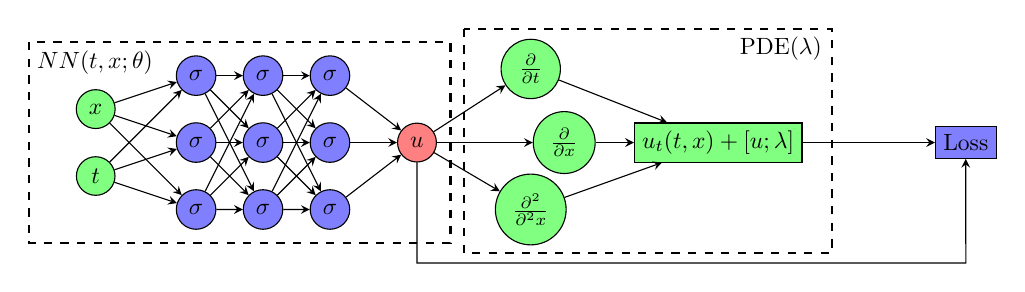
\begin{tikzpicture}[
      % Define styles
      neuron/.style={circle,draw,minimum size=.2cm},
      func/.style={rectangle,draw,minimum size=.2cm},
      PDE/.style={func, fill=green!50},
      loss/.style={func, fill=blue!50},
      input/.style={neuron, fill=green!50},
      hidden/.style={neuron, fill=blue!50},
      output/.style={neuron, fill=red!50},
      diff/.style={neuron, fill=green!50},
      arrow/.style={->,>=stealth},
      scale=0.85,
      transform shape
    ]
      
    \steporfull<3->{
      % Input Layer
      \draw[dashed, thick] (-1,0) rectangle (5.3,-3); % 前两个坐标为矩形左下角的坐标,后两个坐标为矩形右上角的坐标
      \node at (-1,0) [below right] {$NN(t,x; \theta)$}; % 文本内容为"文本",位置为方框的左上角

      \node[input] (Input0) at (0,-1) {$x$};
      \node[input] (Input) at (0,-2) {$t$};
    
      % Hidden Layer 1
      \node[hidden] (Hidden11) at (1.5,-0.5) {$\sigma$};
      \node[hidden] (Hidden12) at (1.5,-1.5) {$\sigma$};
      \node[hidden] (Hidden13) at (1.5,-2.5) {$\sigma$};
    
      % Hidden Layer 2
      \node[hidden] (Hidden21) at (2.5,-0.5) {$\sigma$};
      \node[hidden] (Hidden22) at (2.5,-1.5) {$\sigma$};
      \node[hidden] (Hidden23) at (2.5,-2.5) {$\sigma$};
    
      % Hidden Layer 3
      \node[hidden] (Hidden31) at (3.5,-0.5) {$\sigma$};
      \node[hidden] (Hidden32) at (3.5,-1.5) {$\sigma$};
      \node[hidden] (Hidden33) at (3.5,-2.5) {$\sigma$};

      % Output Layer
      \node[output] (Output) at (4.8,-1.5) {$u$};

      % Connect neurons Input-Hidden Layer 1
      \foreach \i in {1,2,3}
          \draw[arrow] (Input) -- (Hidden1\i);
        \foreach \i in {1,2,3}
          \draw[arrow] (Input0) -- (Hidden1\i);
    
      % Connect neurons Hidden Layer 1-Hidden Layer 2
      \foreach \i in {1,2,3}
          \foreach \j in {1,2,3}
              \draw[arrow] (Hidden1\i) -- (Hidden2\j);
    
      % Connect neurons Hidden Layer 2-Hidden Layer 3
      \foreach \i in {1,2,3}
          \foreach \j in {1,2,3}
              \draw[arrow] (Hidden2\i) -- (Hidden3\j);
    
      % Connect neurons Hidden Layer 3-Output
      \foreach \i in {1,2,3}
          \draw[arrow] (Hidden3\i) -- (Output);
    % }

    % \steporfull<2->{
      \draw[dashed, thick] (5.5,0.2) rectangle (11,-3.15);
      \node at (9.5,0.2) [below right] {PDE($\lambda$)}; % 文本内容为"文本",位置为方框的左上角
    %   % Partial Derivatives
      \node[diff] (D1) at (6.5,-0.4) {$\frac{\partial}{\partial t}$};
      \node[diff] (D2) at (7,-1.5) {$\frac{\partial}{\partial x}$};
      \node[diff] (D3) at (6.5,-2.5) {$\frac{\partial^2}{\partial^2 x}$};
      \node[PDE] (PDE) at (9.3,-1.5) {$u_t(t,x) + \varGamma \left[u; \lambda \right]$};

      \foreach \i in {1,2,3}
          \draw[arrow] (Output) -- (D\i);
      \foreach \i in {1,2,3}
          \draw[arrow] (D\i) -- (PDE);
    }

    % \steporfull<2->{
      \node[loss] (L) at (13,-1.5) {Loss};

      \draw[arrow] (Output) |- (13,-3.3) -- (L.south);
      \draw[arrow] (PDE.east) |- (L);
    % }
    \end{tikzpicture}
    \caption{PINN, with with 3 fully connected hidden layers}
    \label{}
\end{figure}
\end{frame}



\begin{frame}
  \frametitle{Introduction}
  \framesubtitle{Recap - Conclusion}
  \begin{block}{Comparing With Finite Difference Time Domain Method (FDTD)}
    \begin{enumerate}
      \item Deep Neural Network \cite{FIRST}
            \begin{itemize}
              \item Gives lower quality approximations.
              \item Takes longer time to train.
              \item Possible to solve high dimension PDEs \vspace*{1em}
            \end{itemize}
      \item Physics Informed Neural Network
            \begin{itemize}
              \item Gives higher quality approximations.
              \item Takes longer time to train.         
              \item Has more flexible way to get results.
              \item Possible to solve high dimension PDEs
            \end{itemize}
    \end{enumerate}    
  \end{block}
\end{frame}


\subsection{Challenges \& Objectives}



\begin{frame}
  \frametitle{Objectives}
  \begin{block}{Project Objectives}
    \begin{enumerate}
      \item Implement FDTD and PINN in \texttt{C++/C}.
      \item Implement FDTD hybrid parallel version using \texttt{MPI/OpenMP}.
      \item Implement PINN GPU parallel version using \texttt{Libtorch/CUDA}.
      \item Optimize performance through parallel computing frameworks.
      \item Evaluate the efficiency and accuracy of FDTDs and PINNs.
    \end{enumerate}
  \end{block}
\end{frame}


\begin{frame}
  \frametitle{Challanges}
  \begin{block}{}
    \begin{enumerate}
      \item Difficulty in modeling and predicting inhomogeneous cascades of scales.
      \item High computational costs and uncertainties in classical methods.
    \end{enumerate}    
  \end{block}
\end{frame}


% \begin{frame}
%   \frametitle{Highlights}
%   \begin{enumerate}
%     \item Utilizing Meta-programming to implement a Templated N-Dimensional Matrix Class.
%     \item Enhancing efficiency, memory management, and computational accuracy
%     \item MPI Topology Environment Based on the Templated Class which provides Convenient array distribution and ghost exchange routines.
%     \item User-friendly interface for researchers
%     \item Implementation of PDE Solvers with Different Parallel Strategies
%     \item GPU-Accelerated PINNs using Libtorch and CUDA.
%   \end{enumerate}
% \end{frame}